\setlength{\columnsep}{3pt}
\begin{flushleft}


\begin{itemize}
	\item The priority value is the process’s actual priority used by the Linux kernel to schedule a task.
	\item Priorities are 0 to 139 in which \textbf{0 to 99} is for real-time and \textbf{100 to 139} for users.
	\begin{figure}[h!]
		\centering
		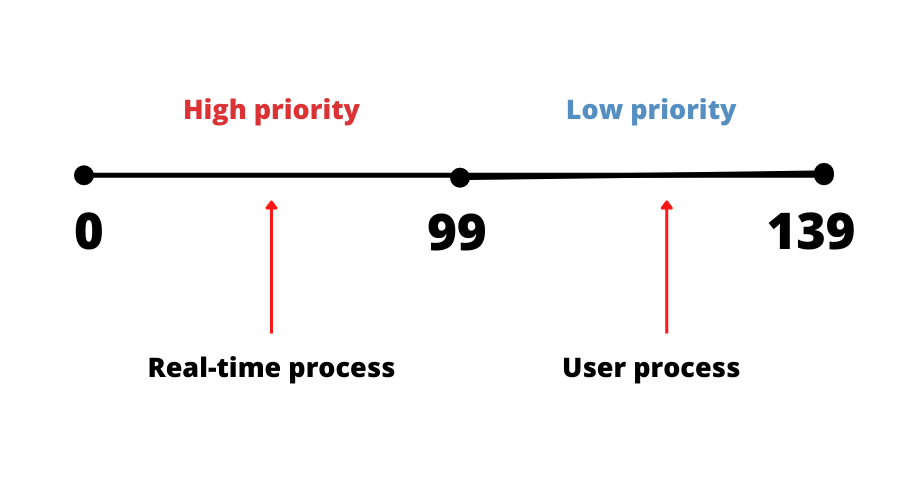
\includegraphics[scale=.4]{content/chapter12/images/pr.png}
		\caption{Priority values}
		\label{fig:cpu5}
	\end{figure}

	Command to check priority of process:
	\bigskip
	\begin{tcolorbox}[breakable,notitle,boxrule=-0pt,colback=pink,colframe=pink]
		\color{black}
		\fontdimen2\font=9pt
		Syntax: top
		\fontdimen2\font=4pt
	\end{tcolorbox}	
	Eg:
	\begin{figure}[h!]
		\centering
		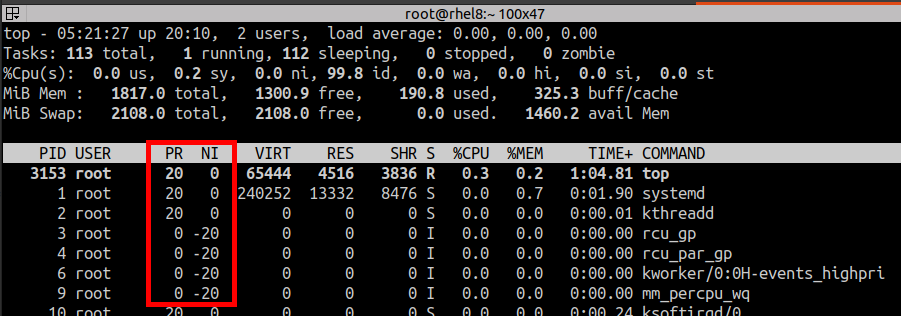
\includegraphics[scale=.32]{content/chapter12/images/nice_1.png}
		\caption{Priority values}
		\label{fig:cpu5}
	\end{figure}
		
	
\end{itemize}

\newpage

\paragraph{How to start a process with a higher or lower priority than default priority?}
\begin{itemize}
	\item \textbf{Solution: Nice value}
	\item Regular user can change priorities of their own jobs.
	\item Priorities assigned by regular user is known as \textbf{‘niceness’}.
	\item The nice value range is -20 to +19 where \textbf{-20 is highest, 0 default and +19 is lowest}.
	\begin{figure}[h!]
		\centering
		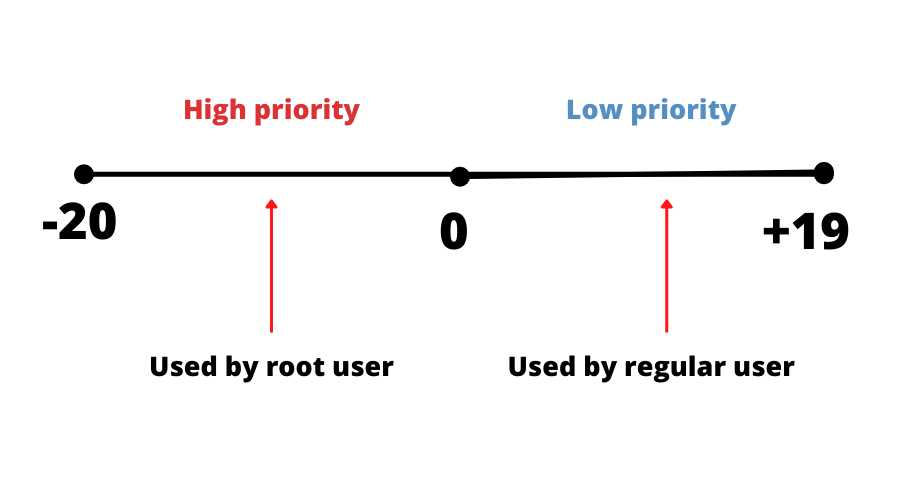
\includegraphics[scale=.5]{content/chapter12/images/nice.png}
		\caption{Nice priority values}
		\label{fig:cpu58}
	\end{figure}
	
	Command to check priority \& nice value of process:
	\bigskip
	\begin{tcolorbox}[breakable,notitle,boxrule=-0pt,colback=pink,colframe=pink]
		\color{black}
		\fontdimen2\font=9pt
		Syntax: ps -eo user,priority,nice,comm | grep command\_name
		\fontdimen2\font=4pt
	\end{tcolorbox}	
	
	Eg:
	\begin{figure}[h!]
		\centering
		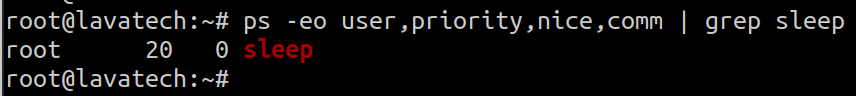
\includegraphics[scale=.4]{content/chapter12/images/ps_nice.png}
		\caption{Sample output}
		\label{fig:cpu589}
	\end{figure}
	\newpage

\end{itemize}



\paragraph{Running a command through the ‘nice’ command}
\begin{itemize}
	\item nice: Run a program with modified scheduling priority.
	\bigskip
	\begin{tcolorbox}[breakable,notitle,boxrule=-0pt,colback=pink,colframe=pink]
		\color{black}
		\fontdimen2\font=9pt
		Syntax: nice -n level command
		\fontdimen2\font=4pt
	\end{tcolorbox}	
	 Eg:
 	\begin{figure}[h!]
	 	\centering
	 	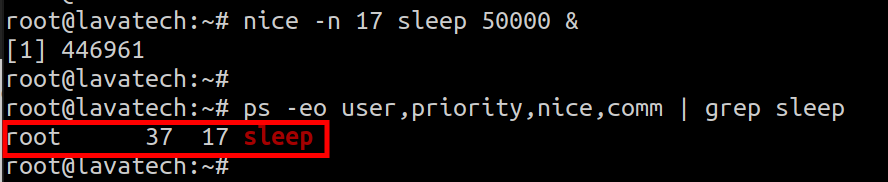
\includegraphics[scale=.4]{content/chapter12/images/noce_2.png}
	 	\caption{Sample output}
	 	\label{fig:cpu5893}
	 \end{figure}
	 
	 \textbf{The relation between nice value and priority is:}
	 \bigskip
	 \begin{tcolorbox}[breakable,notitle,boxrule=-0pt,colback=pink,colframe=pink]
	 	\color{black}
	 	\fontdimen2\font=9pt
	 	Formula: Priority\_value = Nice\_value + 20
	 	\fontdimen2\font=4pt
	 \end{tcolorbox}	 
 	Notice in the above screenshot, priority is 17+20 which is 37.
\end{itemize}

\newpage
\paragraph{How to change the priority of a running process?}
\begin{itemize}
	\item \textbf{Solution: renice command}
	\item renice: Alter priority of running processes.
	\bigskip
	\begin{tcolorbox}[breakable,notitle,boxrule=-0pt,colback=pink,colframe=pink]
		\color{black}
		\fontdimen2\font=9pt
		Syntax: renice -n level PID
		\fontdimen2\font=4pt
	\end{tcolorbox}	
	Eg:
	\bigskip
	\begin{tcolorbox}[breakable,notitle,boxrule=-0pt,colback=black,colframe=black]
		\color{green}
		\fontdimen2\font=9pt
		\# renice -n 15 446961
		\fontdimen2\font=4pt
	\end{tcolorbox}
	\bigskip
	\begin{figure}[h!]
		\centering
		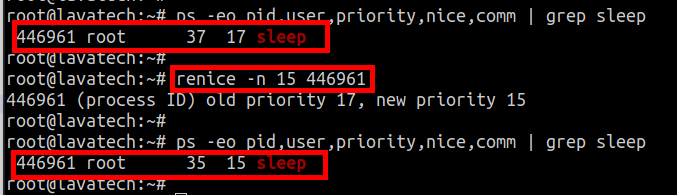
\includegraphics[scale=.5]{content/chapter12/images/renice.png}
		\caption{Sample output}
		\label{fig:cpu58934}
	\end{figure}
	
\end{itemize}




\end{flushleft}

\newpage


